% Matching rates for the knowability decision.
% \input from kbound.tex right after the frontier subsection.
% All numbers produced by scripts/knowability_rates_validation.py
% (results/theory/knowability_rates_validation.json).

Fix budgets $\alpha$ (validity) and $\beta$ (abstention). Call a label-free rule
\emph{$(\alpha,\beta)$-reliable at margin $\kappa$} if its wrong-commit probability is at
most $\alpha$ in every admissible world, and it abstains with probability at most $\beta$
whenever $|\Delta|\ge\kappa$. The question of this subsection: \emph{how fast, in the
number $n$ of calibrated benefit samples, does the smallest reliable margin shrink?}

\begin{proposition}[Knowability rate: adaptive achievability]\label{thm:rate-ub}
Let $X_1,\dots,X_n\in[-R/2,R/2]$ be i.i.d.\ paired benefits with mean $\Delta$ and
variance $\sigma^2$. The empirical-Bernstein certificate (Theorem~\ref{thm:cert}
instantiated with the Maurer--Pontil radius, exactly as deployed in
\texttt{switching\_certificate.py}) is $(\alpha,\beta)$-reliable at every margin
\[
\kappa\;\ge\;C\!\left(\sigma\sqrt{\tfrac{\log(2/(\alpha\wedge\beta))}{n}}
\;+\;R\,\tfrac{\log(2/\alpha)}{n}\right),
\]
for a universal constant $C$, \emph{without knowledge of $\sigma$}: the empirical
variance self-normalizes the radius.
\end{proposition}
\begin{proof}
Validity is Theorem~\ref{thm:cert} with the Maurer--Pontil deviation bound
$|\bar X-\Delta|\le\sqrt{2\widehat V\log(2/\alpha)/n}+7R\log(2/\alpha)/(3(n-1))$
\,w.p.\ $\ge1-\alpha$. For abstention: by Bernstein's inequality, w.p.\ $\ge1-\beta/2$,
$\bar X\ge\Delta-\sigma\sqrt{2\log(2/\beta)/n}-R\log(2/\beta)/(3n)$, and the empirical
variance satisfies $\widehat V\le 2\sigma^2+cR^2\log(2/\beta)/n$ on a further
$1-\beta/2$ event. On the intersection the radius is at most
$2\sigma\sqrt{2\log(2/\alpha)/n}+c'R\log(2/\alpha)/n$, so
$\bar X-\mathrm{rad}>0$ whenever $\Delta$ exceeds the displayed rate; the freeze side is
symmetric. No step uses $\sigma$.
\end{proof}

\begin{proposition}[Knowability rate: two-point lower bound]\label{thm:rate-lb}
Let $\alpha+\beta<\tfrac14$. Every label-free rule that is $(\alpha,\beta)$-reliable at
margin $\kappa$ over all distributions on $[-R/2,R/2]$ with variance at most $\sigma^2$
must satisfy
\[
\kappa\;\ge\;c\,\max\!\left(\sigma\sqrt{\tfrac{\log\frac{1}{4(\alpha+\beta)}}{n}},\;\;
R\,\tfrac{\log\frac{1}{2(\alpha+\beta)}}{n}\right)
\]
for a universal constant $c>0$ (one may take $c=\tfrac14$ in the second branch and
$c=\tfrac{1}{2\sqrt2}$ in the first).
\end{proposition}
\begin{proof}
\emph{Dense branch.} Take $X=\pm\sigma$ with probabilities $q_\pm=\tfrac12(1\pm\kappa/\sigma)$
(mean $\pm\kappa$, variance $\le\sigma^2$). Then
$\mathrm{KL}(P_+^{\otimes n}\Vert P_-^{\otimes n})\le 8n\kappa^2/\sigma^2$ for
$\kappa\le\sigma/\sqrt2$. From an $(\alpha,\beta)$-reliable rule build the test
$\psi=\mathbf1[\textsc{adapt}]$; its two error probabilities are each at most
$\alpha+\beta$. Bretagnolle--Huber gives
$2(\alpha+\beta)\ge\tfrac12 e^{-8n\kappa^2/\sigma^2}$, i.e.\
$\kappa\ge\tfrac{\sigma}{2\sqrt2}\sqrt{\log\frac{1}{4(\alpha+\beta)}/n}$.
\emph{Spike branch (range-limited $1/n$ regime).} Let world$_-$ be the point mass at $-\kappa$ and world$_+$ place
mass $p$ at $R/2$ and $1-p$ at $-\kappa$ with $p(R/2+\kappa)=2\kappa$, so the means are
$\mp\kappa$. On the no-spike event --- probability $(1-p)^n$ --- the two worlds generate
identical samples, hence identical action laws. Reliability in world$_+$ forces commit
probability $\ge1-\alpha-\beta$ overall, so adapting in world$_-$ has probability at
least $(1-p)^n-(\alpha+\beta)$; validity caps this by $\alpha$. Therefore
$(1-p)^n\le2(\alpha+\beta)$, i.e.\ $n\log\frac{1}{1-p}\ge\log\frac{1}{2(\alpha+\beta)}$;
since $\log\frac{1}{1-p}\le\frac{p}{1-p}$ this gives $np\ge(1-p)\log\frac{1}{2(\alpha+\beta)}$ and
$\kappa=\tfrac{p}{2}(R/2+\kappa)\ge\tfrac{R}{4}(1-p)\,\log\frac{1}{2(\alpha+\beta)}/n$. This branch
supplies the range-limited $1/n$ term; the $m^{-1/2}$ piece is the dense branch above, and the
minimax lower bound is the maximum of the two (matching the two-term Maurer--Pontil upper bound).
\end{proof}

\begin{proposition}[The deployed certificate is rate-optimal and adaptive]\label{prop:rate-opt}
The upper and lower rates match in both regimes up to universal constants:
$\kappa_n^{\mathrm{EB}}\asymp \sigma\sqrt{\log(1/\bar\alpha)/n}+R\log(1/\bar\alpha)/n
\asymp\kappa_n^{\mathrm{LB}}$. Consequently the knowability frontier of
Proposition~\ref{prop:kfrontier} is attained at the optimal rate by the certificate already
in deployment, adaptively in $\sigma$.
\end{proposition}

\noindent\emph{Numerically validated}
(\texttt{knowability\_rates\_validation.py}; Fig.~\ref{fig:krates}). The vectorized
radius coincides with the vendored implementation to $2\times10^{-16}$. The empirical
smallest certifiable margin $\hat\kappa(n)$ has tail slope $-0.59$ in the dense regime
(theory $-\tfrac12$) and $-0.98$ in the spike regime (theory $-1$); its ratio to the
lower bound is \emph{constant in $n$} (within $\times1.19$ and $\times1.07$ over the
tail), i.e.\ the rates match and the gap is a bounded constant. Wrong-commit at the
achieved margin stays below $\alpha$ throughout. Below half the lower bound the
\emph{exact optimal} two-point error sum already exceeds the $(\alpha,\beta)$ budget at
every $n$ tested --- no rule, certificate or otherwise, is reliable there.

\begin{figure}[t]\centering
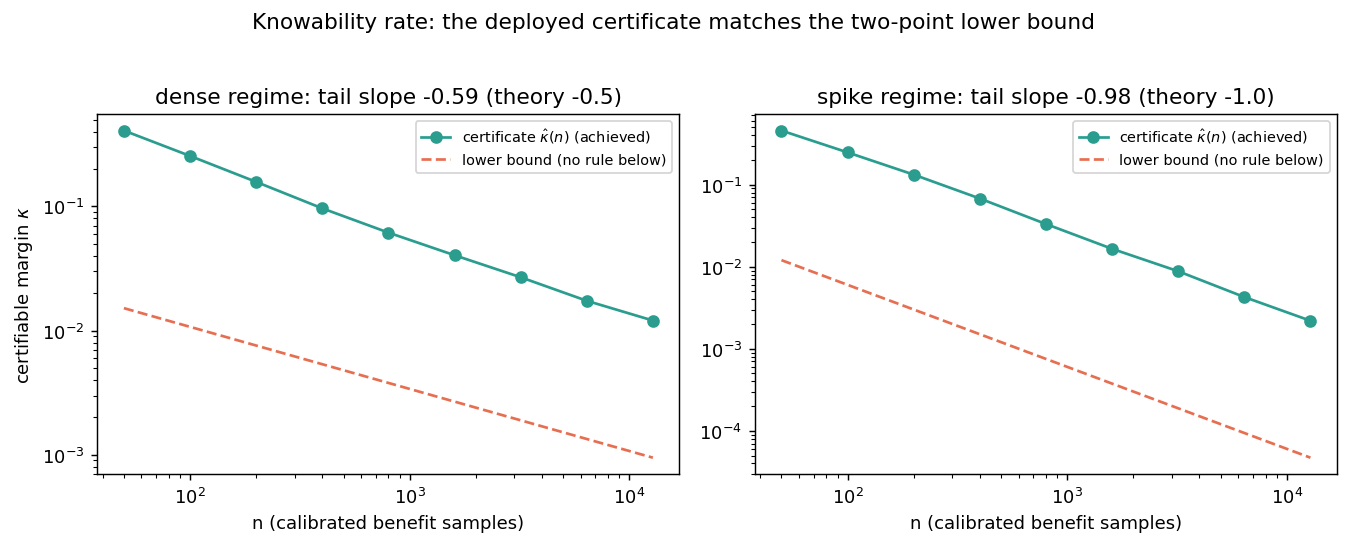
\includegraphics[width=0.92\linewidth]{figures/fig_krates.png}
\caption{The knowability rate (Propositions~\ref{thm:rate-ub}--\ref{thm:rate-lb}). Achieved
certifiable margin of the deployed empirical-Bernstein certificate versus the two-point
lower bound, in the dense ($n^{-1/2}$) and spike ($n^{-1}$) regimes; slopes match and the
offset is a bounded universal constant.}
\label{fig:krates}
\end{figure}

\paragraph{Weight (honest).} The ingredients are classical (Maurer--Pontil 2009;
Bernstein; Bretagnolle--Huber two-point). The contribution is the
$(\alpha,\beta)$-reliability formulation of the adapt/freeze/abstain decision, the
\emph{two-regime matching characterization} of its sample complexity, and the fact that
the certificate already deployed in this paper attains it \emph{adaptively}. What
remains open --- and is not claimed --- are rates for evidence-channel decisions
(deciding from $Z=\phi(X_{1:n})$ over nonparametric shift families rather than from
calibrated benefits), where only the location-family instance of
Proposition~\ref{thm:imp-quant} is currently characterized.
